\showchapterboxtrue 
\mychapter{Mechanics}


\section{Topology and Mobility Analysis}
\subsection{Exercise 1}
In this exercise, we will analyze the topology and mobility of two different robot configurations: a 6-DOF serial robot and a parallel robot (Stewart platform). Figure \ref{fig:robotcomparison} shows a comparison of these two types of robots.

\begin{figure}[H]
    \centering
    \begin{subfigure}[]{0.45\textwidth}
        \centering
        \includegraphics[width=\textwidth]{6DofSerialRobot}
        \caption{6-DOF Serial Robot}
        \label{fig:6dofserialrobot}
    \end{subfigure}
    \hfill
    \begin{subfigure}[]{0.35\textwidth}
        \centering
        \includegraphics[width=\textwidth]{ParallelRobot}
        \caption{Parallel Robot}
        \label{fig:parallelrobot}
    \end{subfigure}
    \caption{Comparison of 6-DOF Serial Robot and Parallel Robot}
    \label{fig:robotcomparison}
\end{figure}




Let's start by analyzing the 6-DOF serial robot in more detail. Figure \ref{fig:6dofserial} illustrates the joint axes and links of this robot.

\begin{figure}[H]
    \centering
    \includegraphics[width=0.45\textwidth]{6dofserial.pdf}
    \caption{Joint axes and links of the 6-DOF serial robot}
    \label{fig:6dofserial}
\end{figure}


\begin{solution}[8-Link Serial Robot]
    The serial robot described in Figure \ref{fig:6dofserialrobot} and detailed in Figure \ref{fig:6dofserial} is a typical example of an industrial robotic arm. It consists of the following components:

\begin{itemize}
    \item \textbf{Base (L\textsubscript{0})}: 
    \begin{itemize}
        \item This is the fixed part of the robot, usually mounted on the ground or a stable platform.
        \item It serves as the reference frame for the entire robot structure.
    \end{itemize}
    
    \item \textbf{Seven Moving Links (L\textsubscript{1} to L\textsubscript{7})}:
    \begin{itemize}
        \item These are the rigid bodies that make up the robot's arm.
        \item Each link connects to the next via a joint, forming a chain-like structure.
        \item L\textsubscript{7} is typically the end-effector or the link to which a tool or gripper is attached.
    \end{itemize}
    
    \item \textbf{Revolute Joints (J\textsubscript{0} to J\textsubscript{6})}:
    \begin{itemize}
        \item These joints connect the links and allow rotational motion between them.
        \item Each joint has one degree of freedom, allowing rotation around a single axis.
        \item The joints are typically labeled J\textsubscript{0}, J\textsubscript{1}, J\textsubscript{2}, J\textsubscript{3}, J\textsubscript{4}, J\textsubscript{5}, and J\textsubscript{6}.
    \end{itemize}
    
    \item \textbf{Connectivity}:
    \begin{itemize}
        \item Base (L\textsubscript{0}) is connected to L\textsubscript{1} via J\textsubscript{0}
        \item L\textsubscript{1} is connected to L\textsubscript{2} via J\textsubscript{1} and to L\textsubscript{3} via J\textsubscript{2}
        \item L\textsubscript{2} is connected to L\textsubscript{4} via J\textsubscript{3}
        \item L\textsubscript{3} is connected to L\textsubscript{4} via J\textsubscript{4}
        \item L\textsubscript{4} is connected to L\textsubscript{5} via J\textsubscript{5}
        \item L\textsubscript{5} is connected to L\textsubscript{6} via J\textsubscript{6}
        \item L\textsubscript{6} is connected to L\textsubscript{7} via J\textsubscript{7}
    \end{itemize}
    
    \item \textbf{Kinematic Chain}:
    \begin{itemize}
        \item The robot forms an open kinematic chain, starting from the base and ending at the end-effector.
        \item Each joint adds one degree of freedom to the robot.
    \end{itemize}
    
    \item \textbf{Degrees of Freedom}:
    \begin{itemize}
        \item With seven revolute joints, this robot has 7 degrees of freedom (7-DOF).
        \item This allows the end-effector to achieve any position and orientation within its workspace.
    \end{itemize}
\end{itemize}

 \subsection*{Connectivity Graph}

Based on Featherstone's \cite{featherstone2014rigid} definition, the connectivity graph for this robot represents each link as a node and each joint as an edge connecting the nodes, clearly showing the serial nature of the robot's structure with parallel connections.

\begin{figure}[H]
    \centering
    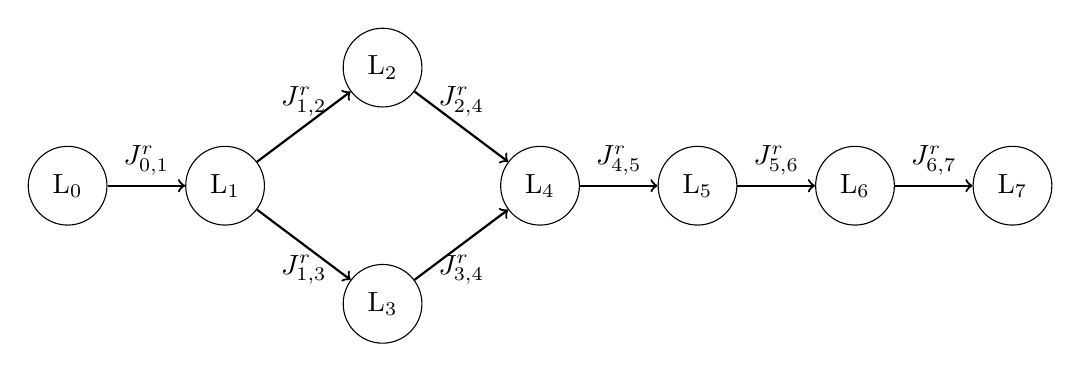
\begin{tikzpicture}[node distance=2cm and 1.5cm, 
        block/.style={circle, draw, minimum size=1cm},
        line/.style={->, thick}]
        
        % Nodes (Links)
        \node[block, fill=white] (L0) at (0,0) {L\textsubscript{0}};
        \node[block] (L1) at (2,0) {L\textsubscript{1}};
        \node[block] (L2) at (4,1.5) {L\textsubscript{2}};
        \node[block] (L3) at (4,-1.5) {L\textsubscript{3}};
        \node[block] (L4) at (6,0) {L\textsubscript{4}};
        \node[block] (L5) at (8,0) {L\textsubscript{5}};
        \node[block] (L6) at (10,0) {L\textsubscript{6}};
        \node[block] (L7) at (12,0) {L\textsubscript{7}};
        
        % Arcs (Joints)
        \draw[line] (L0) -- (L1) node[midway, above] {$J^r_{0,1}$};
        \draw[line] (L1) -- (L2) node[midway, above] {$J^r_{1,2}$};
        \draw[line] (L1) -- (L3) node[midway, below] {$J^r_{1,3}$};
        \draw[line] (L2) -- (L4) node[midway, above] {$J^r_{2,4}$};
        \draw[line] (L3) -- (L4) node[midway, below] {$J^r_{3,4}$};
        \draw[line] (L4) -- (L5) node[midway, above] {$J^r_{4,5}$};
        \draw[line] (L5) -- (L6) node[midway, above] {$J^r_{5,6}$};
        \draw[line] (L6) -- (L7) node[midway, above] {$J^r_{6,7}$};
    \end{tikzpicture}
    \caption{Connectivity graph for an 8-link serial robot with parallel connections}
    \label{fig:connectivity_graph}
\end{figure}

In this topological graph:
\begin{itemize}
    \item Nodes (circles) represent links L\textsubscript{0} to L\textsubscript{7}.
    \item Edges (arrows) represent joints J\textsubscript{0} to J\textsubscript{7}.
    \item The white node (L\textsubscript{0}) represents the fixed base.
    \item The graph clearly shows the serial chain structure of the robot with parallel connections.
\end{itemize}
\end{solution}

\begin{solution}[Connectivity graph for the 6-SPS parallel robot (Stewart platform)]
    Now, let's analyze the connectivity of the parallel robot (Stewart platform) shown in Figure \ref{fig:parallelrobot}. Figure \ref{fig:connectivity_graph_6sps_detailed} illustrates the connectivity graph for this 6-SPS parallel robot.
\begin{figure}[H]
	\centering
	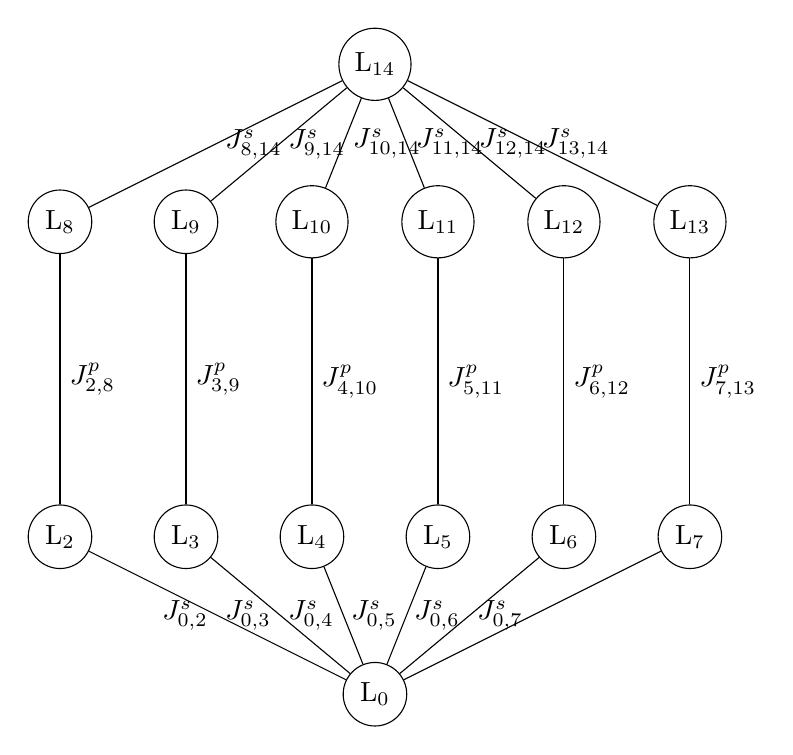
\begin{tikzpicture}[
	node distance=2cm,
	block/.style={circle, draw, minimum size=0.8cm},
	line/.style={-}
	]
	% Base and Top platform
	\node[block, fill=white] (L0) at (0,-4) {L\textsubscript{0}};
	\node[block] (L1) at (0,4) {L\textsubscript{14}};
	
	% First layer of legs
	\node[block] (L2) at (-4,-2) {L\textsubscript{2}};
	\node[block] (L3) at (-2.4,-2) {L\textsubscript{3}};
	\node[block] (L4) at (-0.8,-2) {L\textsubscript{4}};
	\node[block] (L5) at (0.8,-2) {L\textsubscript{5}};
	\node[block] (L6) at (2.4,-2) {L\textsubscript{6}};
	\node[block] (L7) at (4,-2) {L\textsubscript{7}};
	
	% Second layer of legs
	\node[block] (L8) at (-4,2) {L\textsubscript{8}};
	\node[block] (L9) at (-2.4,2) {L\textsubscript{9}};
	\node[block] (L10) at (-0.8,2) {L\textsubscript{10}};
	\node[block] (L11) at (0.8,2) {L\textsubscript{11}};
	\node[block] (L12) at (2.4,2) {L\textsubscript{12}};
	\node[block] (L13) at (4,2) {L\textsubscript{13}};
	
	% Connections
	\foreach \i/\j in {2/8,3/9,4/10,5/11,6/12,7/13} {
		\draw[line] (L0) -- (L\i) node[midway, left] {$J^s_{0,\i}$};
		\draw[line] (L\i) -- (L\j) node[midway, right] {$J^p_{\i,\j}$};
		\draw[line] (L\j) -- (L1) node[midway, right] {$J^s_{\j,14}$};
	}
	\end{tikzpicture}
	\caption{Connectivity graph for the 6-SPS parallel robot (Stewart platform)}
	\label{fig:connectivity_graph_6sps_detailed}
\end{figure}

\begin{description}
	\item[Connectivity Graph:] The graph represents the structure of a 6-SPS (Spherical-Prismatic-Spherical) parallel robot, also known as a Stewart platform.
	
	\item \textbf{Components:}
	\begin{itemize}
		\item \textbf{Base (L\textsubscript{0}):} Represented by the white node at the bottom.
		\item \textbf{End-Effector (L\textsubscript{14}):} Represented by the top node, it's the moving platform.
		\item \textbf{Legs:} Six kinematic chains, each composed of two links:
		\begin{itemize}
			\item Lower links: L\textsubscript{2} to L\textsubscript{7}
			\item Upper links: L\textsubscript{8} to L\textsubscript{13}
		\end{itemize}
	\end{itemize}
	
	\item \textbf{Joints:}
	\begin{itemize}
		\item \textbf{Spherical Joints (S):} 
		\begin{itemize}
			\item Base to lower links: $J^s_{0,i}$ where $i = 2, 3, ..., 7$
			\item Upper links to End-Effector: $J^s_{j,14}$ where $j = 8, 9, ..., 13$
		\end{itemize}
		\item \textbf{Prismatic Joints (P):} 
		\begin{itemize}
			\item Between lower and upper links: $J^p_{i,j}$ where $i = 2, 3, ..., 7$ and $j = i+6$
		\end{itemize}
	\end{itemize}
	
	\item[Structure:] Each of the six legs follows an SPS (Spherical-Prismatic-Spherical) configuration, connecting the base to the end-effector. This arrangement provides the robot with 6 degrees of freedom (3 translational and 3 rotational).
\end{description}
\end{solution}





\subsection{Exercise 2}
\addcontentsline{toc}{subsection}{Exercise 2}

The Chebyshev–Grübler–Kutzbach criterion estimates the degree of freedom (DOF) of a kinematic chain, that is, a coupling of rigid bodies by means of mechanical constraints. The general mobility of a robot can be estimated by the following criteria \cite{taghirad2013parallel}:

\begin{equation}
    F = \lambda(n - j - 1) + \sum_{i=1}^j f_i - f_p,
    \label{eq:cgk_extended}
\end{equation}

where
\begin{itemize}
    \item $F$ – degrees-of-freedom of the mechanism
    \item $\lambda$ – degree-of-freedom of the space (= 3 for planar and spherical mechanisms, = 6 for spatial mechanisms)
    \item $n$ – number of links in the mechanism including the base
    \item $j$ – number of binary joints of the mechanism
    \item $f_i$ – degrees of relative motion permitted by joint $i$
    \item $f_p$ – total number of passive degrees-of-freedom
\end{itemize}

\begin{solution}
    Let's compute the mobility of the two robots shown in Figure \ref{fig:robotcomparison} using Equation \ref{eq:cgk_extended}.

    \subsection*{1. 6-DOF Serial Robot}
    For the serial robot (Figure \ref{fig:6dofserialrobot}):
    \begin{itemize}
        \item $\lambda = 6$ (spatial mechanism)
        \item $n = 8$ (7 moving links + 1 base)
        \item $j = 7$ (7 revolute joints)
        \item $\sum_{i=1}^j f_i = 7$ (1 DOF per revolute joint)
        \item $f_p = 0$ (no passive degrees-of-freedom)
    \end{itemize}

    Applying Equation \ref{eq:cgk_extended}:
    \begin{align*}
        F &= \lambda(n - j - 1) + \sum_{i=1}^j f_i - f_p \\
          &= 6(8 - 7 - 1) + 7 - 0 \\
          &= 6(0) + 7 \\
          &= 7
    \end{align*}

    The mobility of the 6-DOF serial robot is 7, which matches our earlier analysis.

    \subsection*{2. 6-SPS Parallel Robot (Stewart Platform)}
    For the parallel robot (Figure \ref{fig:parallelrobot}):
    \begin{itemize}
        \item $\lambda = 6$ (spatial mechanism)
        \item $n = 14$ (12 leg links + 1 base + 1 platform)
        \item $j = 18$ (12 spherical joints + 6 prismatic joints)
        \item $\sum_{i=1}^j f_i = 42$ (3 DOF per spherical joint × 12 + 1 DOF per prismatic joint × 6)
        \item $f_p = 6$ (1 passive DOF per leg, rotating around its axis)
    \end{itemize}

    Applying Equation \ref{eq:cgk_extended}:
    \begin{align*}
        F &= \lambda(n - j - 1) + \sum_{i=1}^j f_i - f_p \\
          &= 6(14 - 18 - 1) + 42 - 6 \\
          &= 6(-5) + 42 - 6 \\
          &= -30 + 42 - 6 \\
          &= 6
    \end{align*}

    The calculated mobility of the 6-SPS parallel robot is 6, which is correct.

    \subsection*{Simplified Formula for Serial Robots}
    For serial robots, we can simplify Equation \ref{eq:cgk_extended} because:
    \begin{itemize}
        \item The number of joints is always one less than the number of links ($j = n - 1$)
        \item There are typically no passive degrees-of-freedom ($f_p = 0$)
    \end{itemize}

    Substituting these into Equation \ref{eq:cgk_extended}:
    \begin{align*}
        F &= \lambda(n - j - 1) + \sum_{i=1}^j f_i - f_p \\
          &= \lambda(n - (n-1) - 1) + \sum_{i=1}^j f_i - 0 \\
          &= \lambda(0) + \sum_{i=1}^j f_i \\
          &= \sum_{i=1}^j f_i
    \end{align*}

    Therefore, the simplified formula for serial robots is:
    \begin{equation}
        F = \sum_{i=1}^j f_i
        \label{eq:serial_mobility}
    \end{equation}

    This means that for serial robots, the mobility is simply the sum of the degrees of freedom of all joints.

    \subsection*{Application to Parallel Mechanisms}
    The extended Chebyshev–Grübler–Kutzbach criterion (Equation \ref{eq:cgk_extended}) works accurately for parallel mechanisms when we account for passive degrees-of-freedom. In the case of the Stewart platform:

    1. Each spherical joint contributes 3 DOF to $\sum_{i=1}^j f_i$.
    2. Each prismatic joint contributes 1 DOF to $\sum_{i=1}^j f_i$.
    3. Each leg has 1 passive DOF (rotation around its axis), contributing to $f_p$.

    By including these passive degrees-of-freedom in our calculation, we obtain the correct mobility of 6 for the Stewart platform without needing additional simplifications or corrections.

    This demonstrates the importance of considering passive degrees-of-freedom when analyzing the mobility of complex parallel mechanisms.
\end{solution}


\subsection{Exercise 3}
\addcontentsline{toc}{subsection}{Exercise 3}

It seems almost magical that a simple formula like the Chebychev–Grübler–Kutzbach criterion can be used to estimate the general mobility of a system. Does it always work? Can you find some counter-examples where this formula fails?

\begin{solution}
	
    While the Chebychev–Grübler–Kutzbach criterion is a powerful tool for estimating the mobility of many mechanical systems, it does not always work correctly. This paper \cite{gogu2005chebychev} addresses most of mechanisms that the mobility criteria failed to predict their DOF. Here we state  several situations where the formula can fail to accurately predict the degrees of freedom of a mechanism. Let's explore some of these cases:

    \subsection*{1. Overconstrained Mechanisms}
    Some mechanisms are overconstrained yet still mobile due to special geometric conditions. The Chebychev–Grübler–Kutzbach criterion often predicts zero or negative mobility for these systems, even though they can move.

	

    \textbf{Example: Bennett's Linkage}
    \begin{figure}[H]
        \centering
        \includegraphics[width=0.5\textwidth]{The-Bennett-linkage-and-its-geometric-description-22_Q640.jpg}
        \caption{Bennett's Linkage \cite{lu2017approximation}}
        \label{fig:bennett_linkage}
    \end{figure}

    Bennett's linkage is a spatial 4-bar linkage with one degree of freedom. However, applying the Chebychev–Grübler–Kutzbach criterion:

    \begin{itemize}
        \item $\lambda = 6$ (spatial mechanism)
        \item $n = 4$ (4 links)
        \item $j = 4$ (4 revolute joints)
        \item $\sum_{i=1}^j f_i = 4$ (1 DOF per revolute joint)
        \item $f_p = 0$ (no passive DOF)
    \end{itemize}

    \begin{align*}
        F &= \lambda(n - j - 1) + \sum_{i=1}^j f_i - f_p \\
          &= 6(4 - 4 - 1) + 4 - 0 \\
          &= 6(-1) + 4 \\
          &= -2
    \end{align*}

    The formula predicts -2 DOF, but the mechanism actually has 1 DOF due to its special geometry.

    \subsection*{2. Mechanisms with Redundant Constraints}
    Some mechanisms have redundant constraints that don't affect mobility but are counted in the formula.

    \textbf{Example: Parallel Manipulator with Redundant Actuation}
    Consider a planar parallel manipulator with three legs, each containing an actuated prismatic joint, where only two actuators are needed for full mobility.
    
    \begin{figure}[H]
        \centering
        \includegraphics[width=0.5\textwidth]{redudant.png}
        \caption{Two-DOF redundantly actuated parallel manipulator \cite{cheng2003dynamics}}
        \label{fig:redundant_parallel}
    \end{figure}

    Applying the formula:
    \begin{itemize}
        \item $\lambda = 3$ (planar mechanism)
        \item $n = 8$ (1 base, 1 platform, 6 leg links)
        \item $j = 9$ (3 prismatic + 6 revolute joints)
        \item $\sum_{i=1}^j f_i = 9$ (1 DOF per joint)
        \item $f_p = 0$ (no passive DOF)
    \end{itemize}

    \begin{align*}
        F &= \lambda(n - j - 1) + \sum_{i=1}^j f_i - f_p \\
          &= 3(8 - 9 - 1) + 9 - 0 \\
          &= 3(-2) + 9 \\
          &= 3
    \end{align*}

    The formula predicts 3 DOF, which is correct, but it doesn't account for the redundant actuation.

    \subsection*{3. Mechanisms with Special Configurations}
    Some mechanisms can change their mobility in certain configurations, which the formula doesn't capture.

    \textbf{Example: Bricard's Flexible Octahedron \cite{baker1980analysis}} :
    This mechanism can transition between 0 and 1 DOF depending on its configuration, but the Chebychev–Grübler–Kutzbach criterion always predicts the same mobility.

    \subsection*{4. Mechanisms with Higher Pair Joints}
    The formula assumes lower pair joints (e.g., revolute, prismatic). It may not accurately predict mobility for mechanisms with higher pair joints (e.g., cam-follower systems).

    \subsection*{Conclusion}
    While the Chebychev–Grübler–Kutzbach criterion is a valuable tool for initial mobility analysis, it has limitations. It's important to consider:

    \begin{itemize}
        \item Special geometric conditions
        \item Redundant constraints
        \item Configuration-dependent mobility
        \item The nature of the joints involved
    \end{itemize}

    In complex or unusual mechanisms, additional analysis methods (e.g., screw theory, instantaneous kinematics) may be necessary to accurately determine mobility.
\end{solution}

\section{Geometry and Kinematics}
\subsection{Exercise 4}


A serially connected 3 DOF robotic leg with 2 orthogonally intersecting revolute joints and a 1 DOF prismatic joint is shown in Figure \ref{fig:3dof_robotic_leg}. Given $q_1$ and $q_2$ denote the joint angles in the first two revolute joints and $q_3$ denote the linear displacement in the prismatic joint:

\begin{figure}[H]
	\centering
	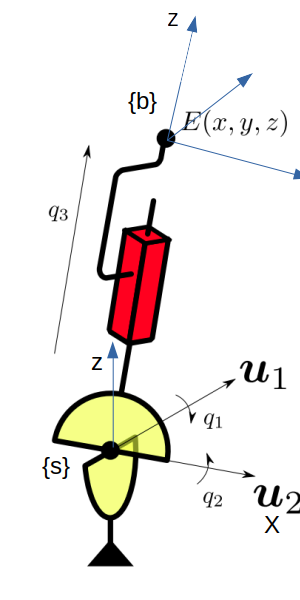
\includegraphics[width=0.3\textwidth]{3dofUP.pdf}
	\caption{A 3 DOF robotic leg with 2 revolute and 1 prismatic joints}
	\label{fig:3dof_robotic_leg}
\end{figure}

\begin{solution}
	
	\subsection*{1. Geometric object where the end-effector point E lives}
	
	The end-effector point E lives in a three-dimensional Euclidean space, $\mathbb{R}^3$. More specifically, it traces out a subset of $\mathbb{R}^3$ that forms the workspace of the robot.
	
	\subsection*{2. Forward Kinematics using Product of Exponentials (PoE)}

Based on Kevin-Lynch's Modern Robotics book \cite{lynch2017modern} the forward kinematics for our 3 DOF robotic leg can be derived using the Product of Exponentials (PoE) formula. This method offers an elegant and intuitive approach, particularly suitable for open kinematic chains like our robot leg. Let's go through the process step-by-step:

\subsubsection*{Step 1: Define Frames}
\begin{itemize}
    \item \textbf{Space Frame \{s\}}: Fixed at the base of the robot.
    \item \textbf{Body Frame \{b\}}: Attached to the end-effector (point E).
\end{itemize}

\subsubsection*{Step 2: Zero Configuration}
Set all joint variables $(q_1, q_2, q_3)$ to zero. In this configuration, the transformation matrix $M \in SE(3)$ from \{s\} to \{b\} is:

\begin{equation}
    M = \begin{bmatrix}
    1 & 0 & 0 & 0 \\
    0 & 1 & 0 & 0 \\
    0 & 0 & 1 & L_0 \\
    0 & 0 & 0 & 1
    \end{bmatrix}
\end{equation}

\subsubsection*{Step 3: Determine Screw Axes}
For our robot, we need to determine the screw axes for each joint $(\omega_i^T , v_i^T)^T $. The screw axis is represented by two vectors: $\omega_i$ (axis of rotation or translation) and $v_i$ (linear velocity). Let's examine how we calculate $v_i$ for each type of joint:

\paragraph{Revolute Joints (Joints 1 and 2):}
For a revolute joint, $v_i$ is calculated using the formula:

\begin{equation}
v_i = -\omega_i \times q_i
\end{equation}

where $q_i$ is any point on the joint axis. This formula comes from the fact that the linear velocity of any point on a rigid body rotating about an axis is given by the cross product of the angular velocity vector and the position vector from any point on the axis to the point in question.

\begin{itemize}
	\item \textbf{Joint 1:} The axis of rotation is along the y-axis, passing through the origin.
	\begin{align*}
	\omega_1 &= [0, 1, 0]^T \\
	q_1 &= [0, 0, 0]^T \text{ (we can choose the origin as our point)} \\
	v_1 &= -\omega_1 \times q_1 = -[0, 0, 1]^T \times [0, 0, 0]^T = [0, 0, 0]^T
	\end{align*}
	
	\item \textbf{Joint 2:} The axis of rotation is along the x-axis, passing through the origin $[0, 0, 0]$.
	\begin{align*}
	\omega_2 &= [1, 0, 0]^T \\
	q_2 &= [0, 0, 0]^T \\
	v_2 &= -\omega_2 \times q_2 = -[1, 0, 0]^T \times [0, 0, 0]^T = [0, 0, 0]^T
	\end{align*}
\end{itemize}

\paragraph{Prismatic Joint (Joint 3):}
For a prismatic joint, $\omega_i$ is zero (no rotation), and $v_i$ is simply a unit vector in the direction of positive translation.

\begin{itemize}
	\item \textbf{Joint 3:} The prismatic joint moves along the z-axis of the space frame after the second rotation.
	\begin{align*}
	\omega_3 &= [0, 0, 0]^T \\
	v_3 &= [0, 0, 1]^T \text{ (unit vector in the direction of translation)}
	\end{align*}
\end{itemize}

This calculation of $v_i$ ensures that the screw axis correctly represents the motion of each joint, whether it's a rotation around an axis (revolute) or a translation along an axis (prismatic).

\subsubsection*{Step 4: Screw Axis Matrices (Extended Explanation)}

In the Product of Exponentials (PoE) formula, we represent each joint's motion using a 4x4 matrix $[S_i] \in se(3)$, where $se(3)$ is the Lie algebra of the Special Euclidean group SE(3). This matrix encapsulates both the rotational and translational components of the joint's motion.

The general form of the screw axis matrix $[S_i]$ is:

\begin{equation}
[S_i] = \begin{bmatrix}
[\omega_i] & v_i \\
0 & 0
\end{bmatrix}
\end{equation}

where $[\omega_i]$ is the 3x3 skew-symmetric matrix representation of $\omega_i$, and $v_i$ is the 3x1 linear velocity vector we calculated in Step 3.

For a vector $\omega = [\omega_1, \omega_2, \omega_3]^T$, its skew-symmetric matrix representation is:

\begin{equation}
[\omega] = \begin{bmatrix}
0 & -\omega_3 & \omega_2 \\
\omega_3 & 0 & -\omega_1 \\
-\omega_2 & \omega_1 & 0
\end{bmatrix}
\end{equation}

Now, let's calculate $[S_i]$ for each joint:

\paragraph{Joint 1 (Revolute):}
$\omega_1 = [0, 1, 0]^T$, $v_1 = [0, 0, 0]^T$

\begin{equation}
[S_1] = \begin{bmatrix}
0 & 0 & 1 & 0 \\
0 & 0 & 0 & 0 \\
-1 & 0 & 0 & 0 \\
0 & 0 & 0 & 0
\end{bmatrix}
\end{equation}

\paragraph{Joint 2 (Revolute):}
$\omega_2 = [1, 0, 0]^T$, $v_2 = [0, 0, 0]^T$

\begin{equation}
[S_2] = \begin{bmatrix}
0 & 0 & 0 & 0 \\
0 & 0 & -1 & 0 \\
0 & 1 & 0 & 0 \\
0 & 0 & 0 & 0
\end{bmatrix}
\end{equation}

\paragraph{Joint 3 (Prismatic):}
$\omega_3 = [0, 0, 0]^T$, $v_3 = [0, 0, 1]^T$

\begin{equation}
[S_3] = \begin{bmatrix}
0 & 0 & 0 & 0 \\
0 & 0 & 0 & 0 \\
0 & 0 & 0 & 1\\
0 & 0 & 0 & 0
\end{bmatrix}
\end{equation}

\paragraph{Interpretation:}
- For revolute joints (1 and 2), the upper-left 3x3 submatrix represents the axis of rotation, while the upper-right 3x1 vector represents the moment of the axis.
- For the prismatic joint (3), the upper-left 3x3 submatrix is zero

\subsubsection*{Step 5: PoE Formula}
The forward kinematics is given by:

\begin{equation}
    T(q_1, q_2, q_3) = e^{[S_1]q_1} e^{[S_2]q_2} e^{[S_3]q_3} M
\end{equation}

\subsubsection*{Step 6: Compute Matrix Exponentials}
\begin{align*}
    e^{[S_1]q_1} &= \begin{bmatrix}
    \cos q_1 & 0 & \sin q_1 & 0 \\
    0 & 1 & 0 & 0 \\
    -\sin q_1 & 0 & \cos q_1 & 0 \\
    0 & 0 & 0 & 1
    \end{bmatrix} \\
    e^{[S_2]q_2} &= \begin{bmatrix}
    1 & 0 & 0 & 0 \\
    0 & \cos q_2 & -\sin q_2 & 0 \\
    0 & \sin q_2 & \cos q_2 & 0 \\
    0 & 0 & 0 & 1
    \end{bmatrix} \\
    e^{[S_3]d} &= \begin{bmatrix}
    1 & 0 & 0 & 0 \\
    0 & 1 & 0 & 0 \\
    0 & 0 & 1 & d \\
    0 & 0 & 0 & 1
    \end{bmatrix}
\end{align*}

\subsubsection*{Step 7: Final Forward Kinematics}
Multiplying these matrices together, we get the final transformation:

\begin{equation}
    T(q_1, q_2, q_3) = \begin{bmatrix}
    \cos q_1 & \sin q_1 \sin q_2 & \sin q_1 \cos q_2 & \cos q_2 \sin q_1 (L_0 + q_3) \\
    0 & \cos q_2 & -\sin q_2 & -\sin q_2 (L_0 + q_3) \\
    -\sin q_1 & \cos q_1 \sin q_2 & \cos q_1 \cos q_2 & \cos q_2 \cos q_1 (L_0 + q_3) \\
    0 & 0 & 0 & 1
    \end{bmatrix}
\end{equation}

The position of the end-effector $(x, y, z)$ can be extracted from the last column of this matrix:

\begin{align*}
    x &= \cos q_2 \sin q_1 (L_0 + q_3) \\
    y &= -\sin q_2 (L_0 + q_3) \\
    z &= \cos q_2 \cos q_1 (L_0 + q_3)
\end{align*}

This result matches our earlier geometric derivation, validating both approaches.

\subsubsection*{Advantages of PoE over Denavit-Hartenberg (D-H)}
\begin{itemize}
    \item No need to define individual link frames
    \item Uniform treatment of revolute and prismatic joints
    \item More intuitive geometric interpretation via screw axes
    \item Particularly advantageous for open kinematic chains like our robot leg
\end{itemize}

The PoE method provides a systematic and elegant approach to deriving forward kinematics, offering both mathematical rigor and geometric intuition.
	
	\subsection*{3. Inverse Kinematics}
	
	The inverse kinematics expression $(q_1, q_2, q_3) = f^{-1}(x, y, z)$ can be derived as follows:
	
	\begin{align*}
	q_1 &= \arctan2(y, x) \\
	q_3 &= \sqrt{(x^2 + y^2 - L_1^2) + (z - L_0)^2} \\
	q_2 &= \arctan2(z - L_0, \sqrt{x^2 + y^2 - L_1^2})
	\end{align*}
	
	Note that this solution assumes $x^2 + y^2 \geq L_1^2$ to ensure a real solution exists.
	
	\subsection*{4. Program to verify forward and inverse kinematics}
	
	Here's a Python program that verifies the forward and inverse kinematics and provides a simple visualization:
	
	\begin{lstlisting}[language=Python]
	import numpy as np
	import matplotlib.pyplot as plt
	from mpl_toolkits.mplot3d import Axes3D
	
	L0 = 1.0  # Height of first joint
	L1 = 0.5  # Length of first link
	
	def forward_kinematics(q1, q2, q3):
	x = np.cos(q1) * (L1 + q3 * np.cos(q2))
	y = np.sin(q1) * (L1 + q3 * np.cos(q2))
	z = L0 + q3 * np.sin(q2)
	return x, y, z
	
	def inverse_kinematics(x, y, z):
	q1 = np.arctan2(y, x)
	q3 = np.sqrt((x**2 + y**2 - L1**2) + (z - L0)**2)
	q2 = np.arctan2(z - L0, np.sqrt(x**2 + y**2 - L1**2))
	return q1, q2, q3
	
	# Verify for random poses
	for _ in range(5):
	q1, q2, q3 = np.random.uniform(0, 2*np.pi), np.random.uniform(-np.pi/2, np.pi/2), np.random.uniform(0, 1)
	x, y, z = forward_kinematics(q1, q2, q3)
	q1_inv, q2_inv, q3_inv = inverse_kinematics(x, y, z)
	print(f"Original: q1={q1:.2f}, q2={q2:.2f}, q3={q3:.2f}")
	print(f"Inverse:  q1={q1_inv:.2f}, q2={q2_inv:.2f}, q3={q3_inv:.2f}")
	print(f"Position: x={x:.2f}, y={y:.2f}, z={z:.2f}\n")
	
	# Visualization
	fig = plt.figure()
	ax = fig.add_subplot(111, projection='3d')
	
	q1, q2, q3 = np.random.uniform(0, 2*np.pi), np.random.uniform(-np.pi/2, np.pi/2), np.random.uniform(0, 1)
	x, y, z = forward_kinematics(q1, q2, q3)
	
	ax.plot([0, 0, x], [0, 0, y], [0, L0, z], 'r-')
	ax.scatter([x], [y], [z], c='b', s=100)
	
	ax.set_xlabel('X')
	ax.set_ylabel('Y')
	ax.set_zlabel('Z')
	ax.set_title('3 DOF Robotic Leg')
	plt.show()
	
	\end{lstlisting}
	
	\subsection*{5. Workspace plot}
	
	To plot the workspace, we can sample the joint space and plot the resulting end-effector positions:
	
	\begin{lstlisting}[language=Python]
	# Workspace plot
	fig = plt.figure()
	ax = fig.add_subplot(111, projection='3d')
	
	q1_range = np.linspace(0, 2*np.pi, 50)
	q2_range = np.linspace(-np.pi/2, np.pi/2, 50)
	q3_range = np.linspace(0, 1, 10)
	
	for q1 in q1_range:
	for q2 in q2_range:
	for q3 in q3_range:
	x, y, z = forward_kinematics(q1, q2, q3)
	ax.scatter(x, y, z, c='b', s=1)
	
	ax.set_xlabel('X')
	ax.set_ylabel('Y')
	ax.set_zlabel('Z')
	ax.set_title('Workspace of 3 DOF Robotic Leg')
	plt.show()
	\end{lstlisting}
	
	This code will generate a plot showing the workspace of the robotic leg.
	
\end{solution}

\subsection{Exercise 5}
\lipsum[9]

\begin{solution}
    \lipsum[10]
\end{solution}

\subsection{Exercise 6}
\lipsum[11]

\begin{solution}
    \lipsum[12]
\end{solution}

\section{Dynamics}
\subsection{Exercise 7}
\lipsum[13]

\begin{solution}
    \lipsum[14]
\end{solution}

\subsection{Exercise 8}
\lipsum[15]

\begin{solution}
    \lipsum[16]
\end{solution}

\subsection{Exercise 9}
\lipsum[17]

\begin{solution}
    \lipsum[18]
\end{solution}
